% ===================================================
% CHAPITRE 25 — PÉRIODE CONTEMPORAINE
% Pages imprimées 261-274 — vues 264-277
% ===================================================
\chapter{Période contemporaine}

% --- Page imprimée 261 — vue 264
\begin{center}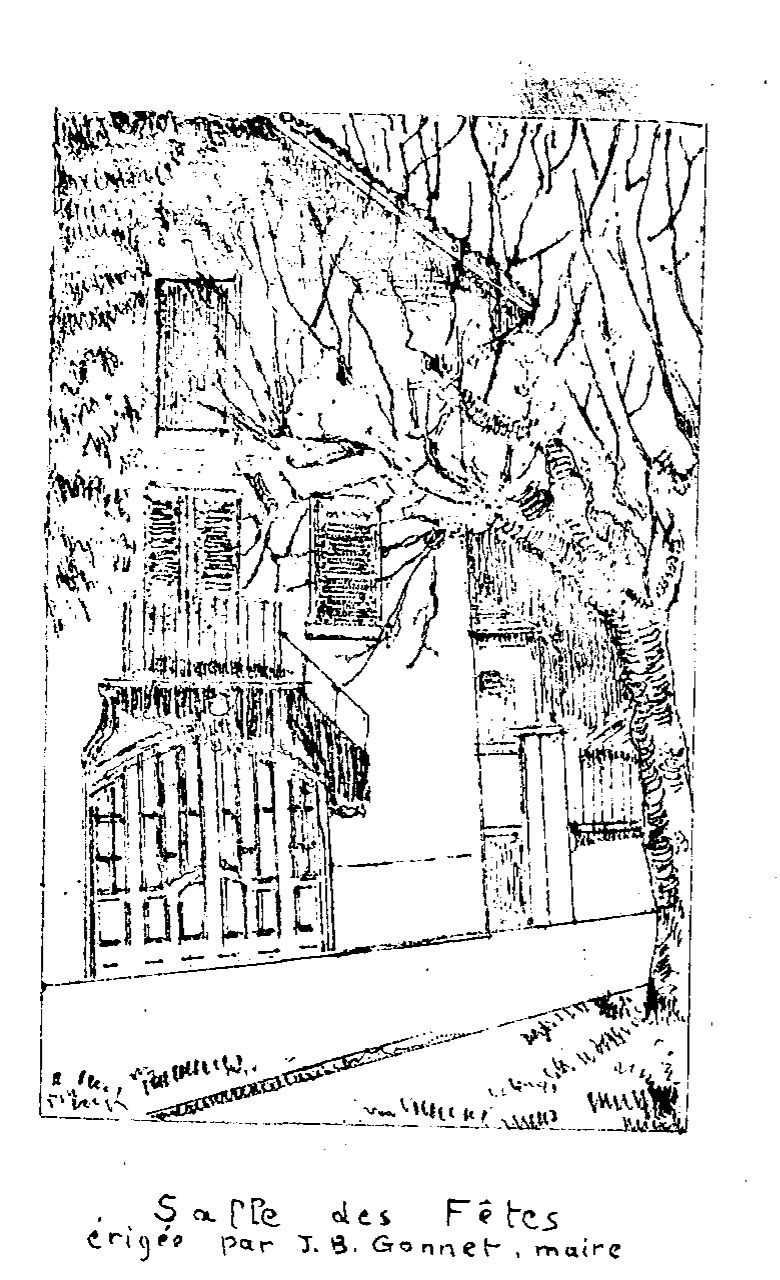
\includegraphics[width=0.62\textwidth]{Illustrations/illus-salle-fetes.jpg}\end{center}

\ourouxlettrine{Illustrations/lettrines/contemporaine.png}{ans ce dernier chapitre de l'Histoire d'Ouroux, que nous avons intitulé « Période contemporaine », il nous reste à parler des quelques événements un peu plus saillants que les autres qui se sont passés au cours de ces 60 dernières années.}

Déjà, en parlant des curés et des Vicaires d'Ouroux, de l'église et des écoles d'Ouroux, nous sommes arrivés jusqu'à nos jours.

D'autres faits, plus ou moins importants, dont nous n'avons pas ou à peine parlé méritent cependant d'être décrits. Nous avons fait appel pour cela à plusieurs témoins oculaires qui racontent eux-mêmes ce qui s'est passé.

% --- Page imprimée 262 — vue 265
\section*{Un bel exemple d'un maire chrétien : Mr Adrien BERLOTY}
\addcontentsline{toc}{section}{Un maire chrétien}

Voici un fait qui se passa en 1897, en une période où le « Laïcisme » était en pleine effervescence. Nous reproduisons ici quelques lignes d'un ouvrage paru sur Adrien BERLOTY, en 1910, et rédigé par un Père Jésuite, ami de la famille.

« En 1897, un épouvantable accident frappa de stupeur la France entière. Dans un grand bazar de charité, à Paris, au moment où la vente battait son plein, et que les salles regorgeaient de monde, un incendie éclata soudain dans l'installation cinématographique. La construction était légère ; elle renfermait quantité de matières inflammables : dans un instant, tout fut en feu. Les issues étaient rares et le dégagement, par conséquent, difficile. Les victimes, hélas, furent nombreuses ; on en compta près de deux cents. Pendant les funérailles, auxquelles Paris presque tout entier s'était porté, le prédicateur de Notre-Dame, le Père Ollivier, monta en chaire et ne craignit pas de parler de la Providence et des châtiments dont elle frappe parfois les nations.

À la séance suivante de la Chambre des Députés, le président, M. Brisson, par manière de réponse aux paroles de l'éloquent dominicain, prononça un discours qui ne fut, d'un bout à l'autre, qu'une insolente négation de Dieu. La Chambre en vota l'affichage dans toutes les communes de France.

Sans permettre de juger qui que ce fut, Adrien Berloty pensa qu'il ne pouvait pas, comme maire d'Ouroux, s'associer aux blasphèmes du sectaire Brisson en permettant l'affichage de son discours. Il ne crut pas non plus que ce fût assez de rester dans une attitude passive ; il voulait d'ailleurs dégager complètement la responsabilité de ses subordonnés et l'assumer lui-même tout entière.

Voici la lettre digne et ferme qu'il écrivit, le 22 mai 1897, au Préfet du Rhône.

\begin{quote}
Monsieur le Préfet,

J'ai l'honneur de vous informer que je ne crois pas devoir faire afficher, à Ouroux, le discours prononcé par M. Brisson, président de la Chambre des Députés, à l'ouverture de la séance du 18 courant. »

% --- Page imprimée 263 — vue 266
Ma conscience se refuse à cet office.

Si je partage pleinement la douleur qui a envahi tous les cœurs à la nouvelle de la catastrophe de la rue Jean-Goujon, je ne peux que réprouver les sentiments de révolte contre Dieu, exprimés à cette occasion par M. Brisson.

L'affichage de ce discours n'a d'autre but que de répandre officiellement ces blasphèmes dans toutes les communes de France. Je ne veux, ni ne puis consentir à me faire le complice de cette besogne, dans la petite commune qui, depuis quatorze ans, me fait l'honneur de me confier ses intérêts.

Les sentiments de ses habitants me sont d'ailleurs trop connus, pour que je ne me rende pas compte que l'affichage de cet outrage à Dieu serait un véritable défi aux croyances religieuses de la population.

Avec mes regrets d'avoir à vous écrire cette lettre, veuillez agréer, Monsieur le Préfet, l'hommage de ma très respectueuse considération.

A. Berloty  \\
Maire de Saint-Antoine d'Ouroux
\end{quote}

Ce n'était pas là un sentiment de vaine forfanterie, encore moins le désir d'attirer sur soi l'attention. Le ton de la lettre l'indique assez et ceux qui connaissaient Adrien Berloty n'en pouvaient douter. C'était simplement le cri de la sentinelle, proposée à la garde d'un camp, et qui, à la vue de l'ennemi, l'arme au bras et sans s'inquiéter des conséquences, répond bravement : « on ne passe pas ! ».

Cet acte courageux ne pouvait demeurer inaperçu. La voix des journaux le publia dans la France entière et les témoignages de sympathie et l'admiration affluèrent de toute part.

C'est d'abord Mgr l'Archevêque de Lyon qui s'exprime par la plume de Mgr Déchelette :

\begin{quote}
« Cher Monsieur et Ami,

Laissez-moi vous féliciter cordialement de votre belle lettre au Préfet du Rhône. Quel bon exemple de vaillance chrétienne vous avez donné, comme toujours.

Les habitants d'Ouroux devront être fiers de leur Maire et ils auront raison. »
\end{quote}

Ce sont des militaires éminents… c'est un collègue… des comités.

La réponse du Préfet fut celle qu'on pouvait attendre. Il suspendit le maire d'Ouroux. Quelques semaines plus tard, la révocation était prononcée au ministère… Pour que personne ne se trompât sur ses intentions, il les expliqua longuement et clairement, dans une lettre à ses administrés au moment de quitter l'exercice de ses fonctions.

% --- Page imprimée 264 — vue 267
\section*{Guerre de 1914--1918  L'Abbé CLEMENT, soldat.}
\addcontentsline{toc}{section}{Guerre 1914--1918}

Nous lisons sur le cahier de délibérations du conseil municipal d'Ouroux ces lignes :

« Grâce au courage de chacun la moisson sera terminée vers les 12 ou 14 Août ; les familles dont les hommes sont mobilisés sont les premières secourues ; une garde civile comprenant tous les hommes valides et quelques femmes est chargée de la surveillance générale et de visiter les maisons isolées, surtout pendant la nuit ; des secours en nature seront distribués aux familles nécessiteuses. Il existe 4 machines à battre le blé dans la commune et sans qu'il soit besoin de les requérir elles seront mises à la disposition des agriculteurs d'Ouroux et des communes limitrophes. La main d'œuvre communale est suffisante pour le moment, mais si le besoin s'en faisait sentir une demande serait adressée à la Préfecture ».

Ce texte nous laisse supposer qu'à Ouroux, après la mobilisation générale, régnait la bonne volonté, l'esprit de solidarité et le patriotisme de toute la population.

Les anciens se souviennent du départ de l'abbé Clément qui fut le dernier vicaire à Ouroux. Il fut un des premiers à partir lors de la mobilisation. Nous relevons, pour vous le raconter, quelques passages d'un discours prononcé par A. SAINT-CYR, aumônier militaire aux 1er et 2ème Zouaves.

« Au moment où sonna le lugubre tocsin de la mobilisation ses premiers mots furent : « Quel malheur ! que de sang versé ! que de larmes ! que de deuils ! ». Il n'hésita pas cependant une minute à remplir son devoir. Mais avant de quitter les fidèles de la paroisse il tenta encore à les édifier par quelques paroles de circonstance pour les prémunir contre le découragement et pour prier une dernière fois pour eux et avec eux. Mr l'Abbé Michard, son vénérable curé, répondant à son pieux désir prépare lui-même la cérémonie des adieux et y invite ses paroissiens. Vu le passage matinal du train que l'Abbé Clément doit prendre aux Ardillats c'est à 3 h ½ du matin qu'a lieu la cérémonie à l'église qui se trouve remplie comme aux grandes solennités : les mobilisés du pays, leurs femmes, leurs enfants, leurs amis, la population tout entière est là, réunie dans un même sentiment de foi. On
% --- Page imprimée 265 — vue 268 (suite)
sent que la guerre, ses dangers et les maux qu'on y endurera en commun ont déjà rapproché les cœurs et réveillé l'esprit chrétien.

L'assistance fait monter ses vœux vers le ciel pour le prêtre aimé qui va nous faire, de son corps, un rempart contre l'invasion de la barbarie allemande et que peut-être on ne reverra plus. Celui-ci offre l'adorable victime pour le salut de la France et le retour de ses frères d'armes qui partent en laissant derrière eux une famille dans les larmes et le besoin. Beaucoup s'approchent de la Table Eucharistique pour y puiser la force et le courage nécessaires au milieu des batailles. Tous prient avec une indicible ferveur. C'est un spectacle on ne peut plus consolant.

La messe terminée, l'Abbé Clément a vite fait d'aller à la sacristie, d'y quitter les ornements sacerdotaux, de prendre son costume de zouave et de revenir ainsi vêtu au milieu du chœur. Là, avec une voix sûre d'elle-même, dans laquelle perce son émotion, il s'adresse à ses camarades de départ. Ses paroles sont plutôt rares et brèves mais combien palpitantes de foi et de patriotisme !…

Les yeux se mouillent de larmes. Des mères, des épouses, des enfants éclatent en sanglots. C'est une scène inoubliable. Mais l'heure presse ; il faut se quitter. Le cher abbé traverse l'église, en serrant la main à ceux de ses frères d'armes qu'il rencontre sur son chemin. Il prend une demi-tasse de café au presbytère et le voilà en route. Le cœur serré, mais rempli de courage, il escalade la montagne, prend le train aux Ardillats et rejoint joyeusement son beau régiment de zouaves à Sathonay… Le 14 septembre, l'Abbé Clément part sur la ligne de feu et dans la nuit du 23 au 24 novembre, à Tracy-le-Val entre 2 et 3 heures du matin il est tué, frappé en pleine tête d'une balle allemande.

Dans ses notes trouvées sur l'Abbé Clément nous relevons ces mots qui nous montrent la piété et le patriotisme de ce prêtre :

« Mon désir serait de continuer mon apostolat auprès des âmes confiées à mes soins. Mais si le Bon Dieu m'appelle à une vie meilleure, ma dernière recommandation sera celle-ci : vous tous qui voulez bien garder de moi un souvenir affectueux, restez unis à Dieu par la Communion fréquente ». Et faisant allusion à la mort qui peut le frapper : « Je meurs content. J'espère au cœur, en donnant rendez-vous au ciel à tous ceux qui ici-bas m'ont demandé de les aider à sauver leur âme ».

% --- Page imprimée 266 — vue 269
La guerre de 1914--1918 fut très meurtrière. Quarante soldats d'Ouroux donnèrent leur vie pour la France. Les noms de tous ces héros sont gravés sur le marbre et la pierre à trois endroits : à l'église, sur le monument aux morts, au cimetière. Les voici tels qu'ils figurent à l'église, sur une plaque de marbre.

\begin{center}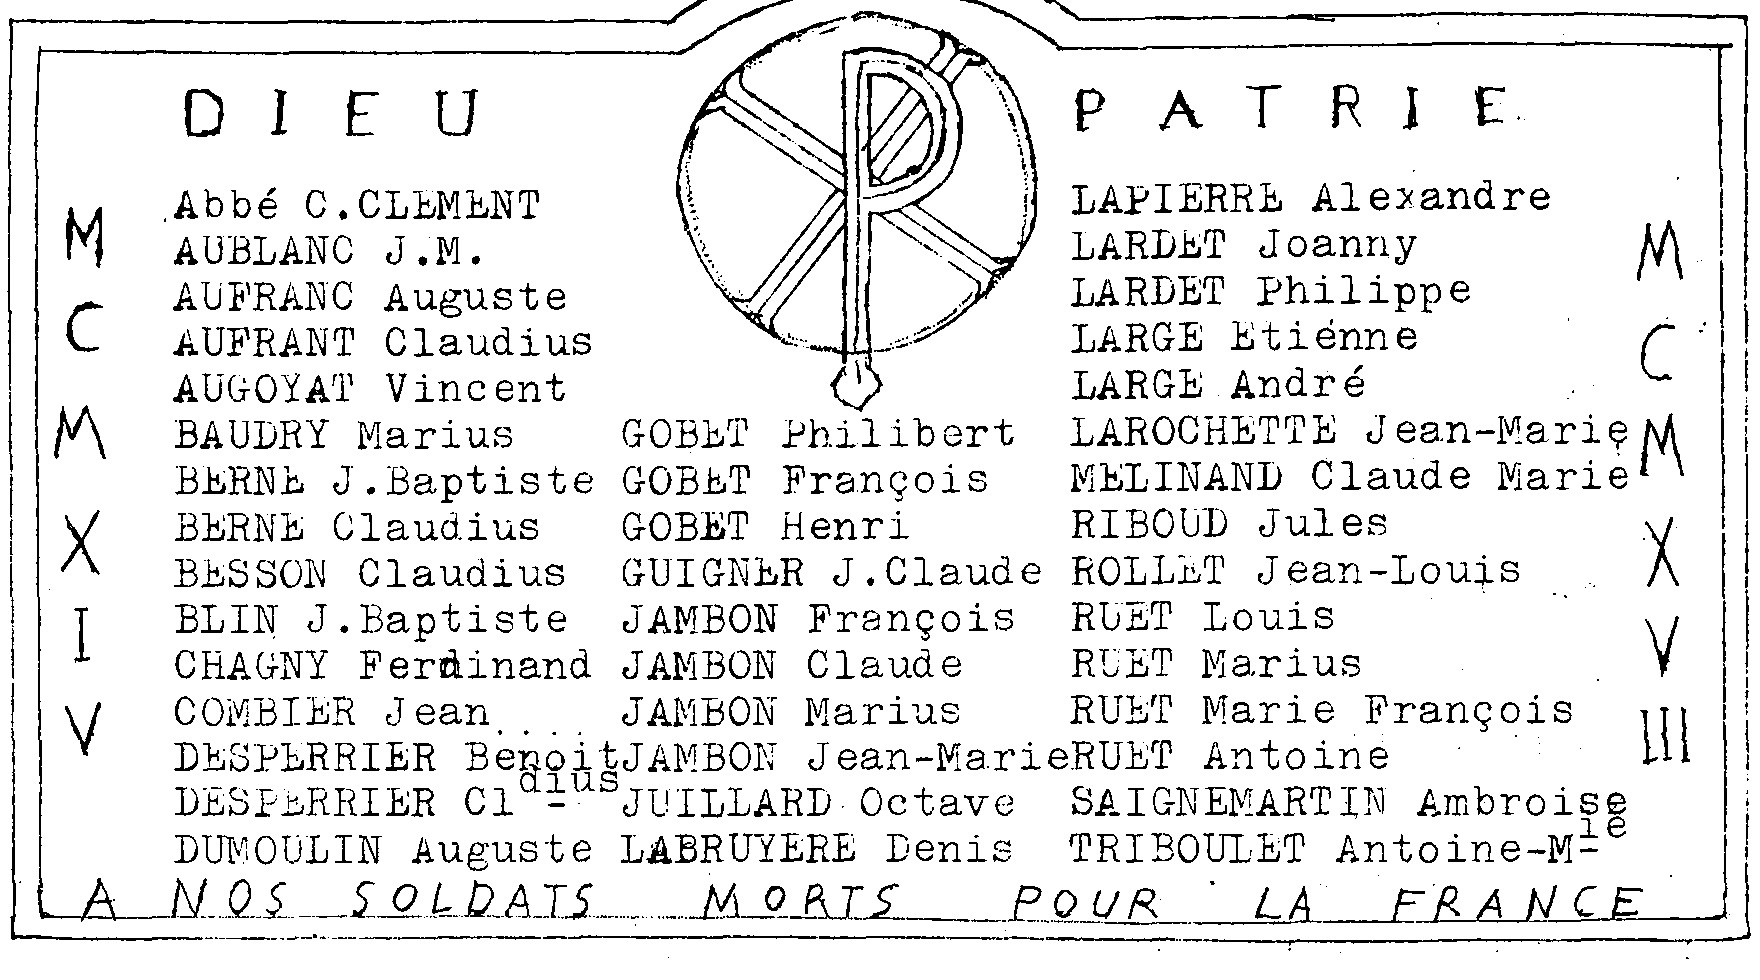
\includegraphics[width=0.62\textwidth]{Illustrations/illus-plaque-soldats.jpg}\end{center}
\iffalse

DIEU                                                                     PATRIE

Abbé C. CLEMENT                                                LAPIERRE Alexandre  
AUBLANC J.M.                                                   LARDET Joanny  
AUFRANC Auguste                                                LARDET Philippe  
AUFRANT Claudius                                               LARGE Étienne  
AUGOYAT Vincent                                                LARGE André  
BAUDRY Marius                                                  LAROCHETTE Jean-Marie  
BERNE J. Baptiste                                              MEINAND Claude Marie  
BERNE Claudius                                                 RIBOUD Jules  
BESSON Claudius                                                ROLLIER Jean-Louis  
BLIN J. Baptiste                                               RUET Louis  
CHAGNY Ferdinand                                               RUET Marius  
COMBIER Jean…                                                  RUET Marie François  
DESPERRIER Benoît                                             RUET Antoine  
DESPERRIER Claudius                                            SAIGNEMARTIN Ambroise  
DUMOULIN Auguste                                               TRIBOULET Antoine-Marie  
GOBET Philibert  
GOBET François  
GOBET Henri  
GUIGNER J. Claude  
JAMBON François  
JAMBON Claude  
JAMBON Marius  
JAMBON Jean-Marie  
JUILLARD Octave  
LABRUYERE Denis

 A NOS SOLDATS MORTS POUR LA FRANCE

\fi
\begin{center}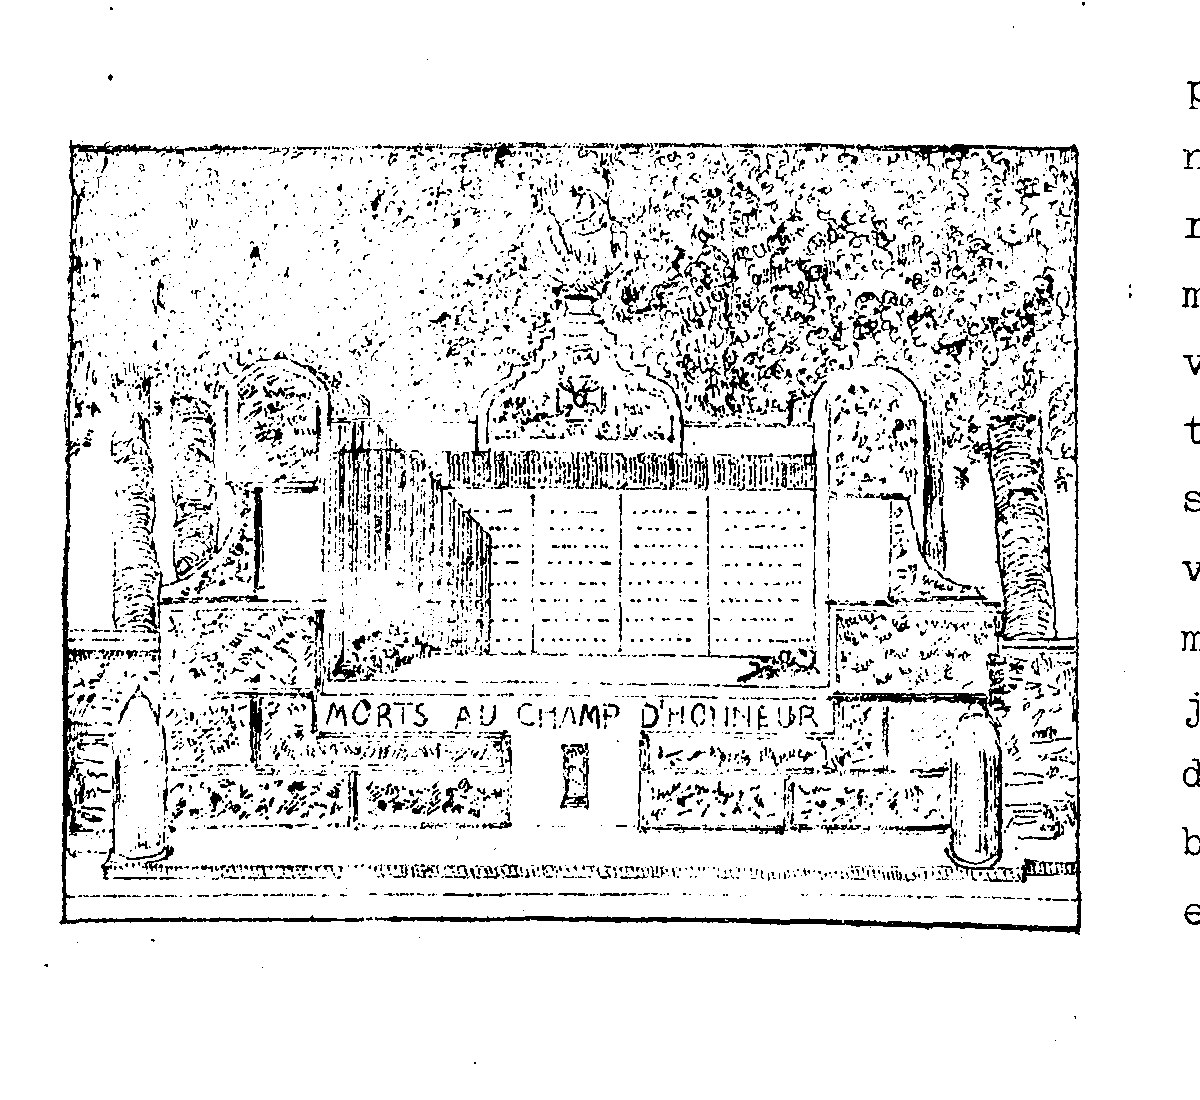
\includegraphics[width=0.62\textwidth]{Illustrations/illus-monument-morts.jpg}\end{center}

En Août 1920 naît le projet d'érection d'un monument aux morts de la guerre. Le devis s'élève à dix mille francs. Le conseil vote 2.000 fr., la souscription publique produit la somme de 7827 frs. Le travail est confié à Mr Myard marbrier-sculpteur de Beaugeu. Mr Riboud a fait don du beau buste de la République de Clésinger qui est d'une grande valeur.

% --- Page imprimée 267 — vue 270
\section*{Catastrophes aériennes (1934 et 1937), par Marius LARGE}
\addcontentsline{toc}{section}{Catastrophes aériennes}

La commune d'Ouroux qui se trouve sur un itinéraire emprunté par de nombreuses compagnies françaises et étrangères a été témoin de deux catastrophes aériennes, l'une militaire, l'autre civile. La première se produisit le 1er septembre 1934. Un avion de chasse, piloté par le lieutenant Georges Vingouroux, faisant partie d'une escadrille de Bron, de retour de Paris, fut contraint, à la suite d'une panne de moteur, de chercher un terrain d'atterrissage. Alors qu'il s'apprêtait à se poser dans un pré appartenant à Mr Gobet de la Forêt, il accrocha des arbres et s'écrasa dans le chemin qui conduit des Jambons à la route de Fontmartin. Le pilote fut tué sur le coup.

La deuxième eut lieu le 24 mars 1937. Effectuant son premier voyage, un hydravion anglais quadrimoteur des Imperial Airway, parti de Southampton pour se rendre en Australie, fut pris, en arrivant dans notre région, dans une tempête de neige, ce qui ne lui permit pas de repérer le bassin du Breuil à Mâcon où il devait faire escale. Perdu dans le brouillard, il vient buter contre le flanc nord-ouest de la montagne de Rochetin, à 500 m de Taboulin. Après avoir raclé le sol pendant 300 m et perdu trois de ses moteurs, il s'arrêta contre des sapins sur le plateau qui, aujourd'hui, porte son nom, le « Capricornus ». Trois membres de l'équipage furent tués sur le coup, un quatrième ainsi que l'unique passagère gravement blessés succombèrent quelques heures après. Seul le radio, moins gravement atteint, réchappa de ce tragique accident qui amena dans notre pays une foule incalculable de curieux venus de tous les coins de France.

\begin{center}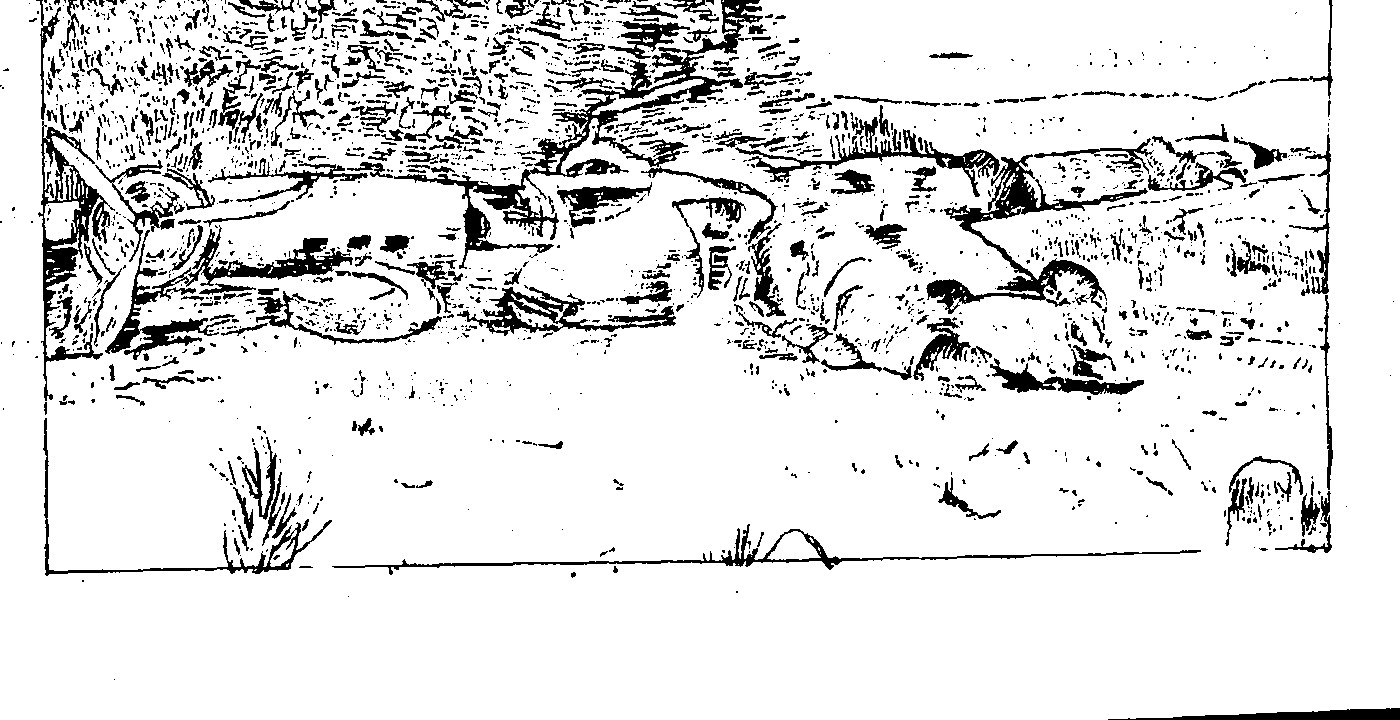
\includegraphics[width=0.62\textwidth]{Illustrations/illus-catastrophe-aerienne.jpg}\end{center}

% --- Page imprimée 268 — vue 271
\section*{Guerre de 1939--1945 — Bombardement d'Ouroux, par Cl. MELINAND}
\addcontentsline{toc}{section}{Guerre 1939--1945 -- bombardement}

« Il était 19 h 30, le 26 juillet 1944 lorsque six avions allemands surgirent du Col de Fontmartin, passèrent au-dessus du village, se dirigèrent du côté de la Serve pour faire subitement demi-tour et revenir sur le village où ils lâchèrent aussitôt de nombreuses bombes explosives et incendiaires. Ces dernières tombèrent dans la montagne des Friats où heureusement le feu ne se propagea pas très vite ; les premières tombèrent dans les bois des Garennes, au-dessus de la ferme des Friats. Les premières bombes explosives qui atteignirent le village tombèrent sur la maison de Mr Lagello, tuant sa femme qui ne devait être remontée des décombres que le lendemain ainsi que Mr Kourlukoff, réfugié de Paris et habitant dans une petite maison accoudée à celle de Mr Lagello. Tout à côté, Mr Desperrier Joanny et Mme Vve Seignemartin, sa voisine, trouvèrent aussi la mort. La fille de Mr Desperrier fut prise sous les décombres et ne fut sortie qu'après deux heures d'effort, blessée à l'épaule. On dut la transporter aussitôt à l'hôpital de Mâcon. Une bombe explosive sur la route devant l'hôtel Desperrier le vida de son contenu ; les maisons de Mr Ruet Antoine, Large Lucien, Large Jean-Marie et l'hôtel Ray furent sérieusement endommagés. Dans sa cuisine Mr Ray fut blessé ainsi que son neveu. D'autres bombes encore tombèrent, démolirent la maison d'habitation et l'atelier de forge de Mr Mélinand, le dépôt de maçonnerie de Mr Bouillard Léon. Une bombe rasa le clocher, tomba derrière l'église endommageant celle-ci et brisant les vitraux.

Pendant le bombardement, les habitants pris de panique se réfugièrent dans le lit de la rivière qui se trouve encaissé ou contre les talus d'un terrain sur « la Ville », à la merci des rafales de mitraille car les avions délestés de leurs bombes mitraillaient tout ce qu'ils voyaient, durant trois quarts d'heure.

Après le bombardement, les pompiers de Tramayes et les gens d'Ouroux arrêtèrent en partie les incendies : une porcherie et un grenier à la ferme des Friats, une écurie et un grenier à la ferme de la Rivière brûlèrent. Seuls furent détruits complètement les garages de Mr Jacquet et de Mr Ray.

On put constater de nombreuses dégradations dans les maisons ainsi que vitres cassées et plusieurs petits dommages ; mais Ouroux ne fut pas détruit complètement car les avions bombardaient par le travers, c'est-à-dire du Château-du-Bois à la ferme des Friats et une bonne partie des bombes explosives tomba dans les prés tuant quelques vaches et moutons appartenant à Mr Fayard.

La nuit vint mettre fin à cette heure terrible qui venait de s'écouler. Cependant un fort orage, au début de la nuit, prolongeait la frayeur qui hantait les esprits.

Tout n'était pas fini, puisque trois semaines après on apprenait la mort affreuse d'un enfant de 11 ans, Ambroise Saignemartin, tué en jouant avec un engin quelconque qui explosa.

La cause de ce bombardement ne fut pas connue. D'après ce que l'on a pu savoir, le jour avant le bombardement un camion contenant une vingtaine d'Allemands fut attaqué par le maquis de Beaujeu. D'après certaine rumeur, en attaquant Ouroux, les Allemands auraient peut-être simplement voulu semer la panique à titre de représaille, pensant que les maquisards pouvaient se trouver dans les bois. C'est la seule raison qui ferait croire au bombardement d'Ouroux puisque le village est entouré de bois.

Le lendemain, Beaujeu fut aussi bombardé, mais il n'y eut qu'un mort et bien moins de dégâts. »

Au cours de cette dernière guerre ces enfants d'Ouroux moururent pour la France. Leurs noms furent joints, à part, sur le monument aux morts, au cimetière et à l'église, dont voici le relevé de la plaque commémorative.

\begin{center}
\setlength{\fboxsep}{6pt}
\fbox{%
\begin{minipage}{0.92\textwidth}
\centering
\textbf{GUERRE 1939 - 1945}\par\medskip
\renewcommand{\arraystretch}{1.08}
\begin{tabular}{@{}p{0.43\linewidth}@{\hspace{0.04\linewidth}}p{0.43\linewidth}@{}}
\textbf{MORTS AU CHAMP D'HONNEUR} & \textbf{VICTIMES DU BOMBARDEMENT}\\
AUCAGNE Jean & du 26 Juillet 1944\\
CHAMPAGNON Jean & DESPERRIER Joanny\\
LUCRUX Raymond & KOURLUKOFF Alexis\\
JAMBON Louis & PASSOT Marie\\
TRICHARD Jean & Veuve SAIGNEMARTIN\\
Déporté politique & PATICHOUD Philomène\\
LAGELLO Georges & Epouse LAGELLO\\
 & SAIGNEMARTIN Ambroise\\[0.4em]
\multicolumn{2}{c}{\textit{Hommage à ceux qui sont morts pour la justice et pour la paix !}}
\end{tabular}
\end{minipage}}
\end{center}
\iffalse
GUERRE 1939 - 1945

MORTS AU CHAMP D'HONNEUR

AUCAGNE Jean  
CHAMPAGNON Jean  
LUCRUX Raymond  
JAMBON Louis  
TRICHARD Jean  

Déporté politique  
LAGELLO Georges  

VICTIMES DU BOMBARDEMENT  
du 26 Juillet 1944

DESPERRIER Joanny  
KOURLUKOFF Alexis  
PASSOT Marie  
Veuve SAIGNEMARTIN  
PATICHOUD Philomène  
Epouse LAGELLO  
SAIGNEMARTIN Ambroise  

Hommage à ceux qui sont morts pour la justice et pour la paix !
\fi

% --- Page imprimée 269 — vue 272
\iffalse
La nuit vint mettre fin à cette heure terrible qui venait de s'écouler. Cependant un fort orage, au début de la nuit, prolongeait la frayeur qui hantait les esprits.

Tout n'était pas fini, puisque trois semaines après on apprenait la mort affreuse d'un enfant de 11 ans, Ambroise Saignemartin, tué en jouant avec un engin quelconque qui explosa.

La cause de ce bombardement ne fut pas connue. D'après ce que l'on a pu savoir, le jour avant le bombardement un camion contenant une vingtaine d'Allemands fut attaqué par le maquis de Beaujeu. D'après certaine rumeur, en attaquant Ouroux, les Allemands auraient peut-être simplement voulu semer la panique à titre de représaille, pensant que les maquisards pouvaient se trouver dans les bois. C'est la seule raison qui ferait croire au bombardement d'Ouroux puisque le village est entouré de bois.

Le lendemain, Beaujeu fut aussi bombardé, mais il n'y eut qu'un mort et bien moins de dégâts. »

Au cours de cette dernière guerre ces enfants d'Ouroux moururent pour la France. Leurs noms furent joints, à part, sur le monument aux morts, au cimetière et à l'église, dont voici le relevé de la plaque commémorative.

GUERRE 1939 - 1945

MORTS AU CHAMP D'HONNEUR

AUCAGNE Jean  
CHAMPAGNON Jean  
LUCRUX Raymond  
JAMBON Louis  
TRICHARD Jean  

Déporté politique  
LAGELLO Georges  

VICTIMES DU BOMBARDEMENT  
du 26 Juillet 1944

DESPERRIER Joanny  
KOURLUKOFF Alexis  
PASSOT Marie  
Veuve SAIGNEMARTIN  
PATICHOUD Philomène  
Epouse LAGELLO  
SAIGNEMARTIN Ambroise  

Hommage à ceux qui sont morts pour la justice et pour la paix !
\fi

% --- Page imprimée 270 — vue 273
\section*{Démolition de vieilles maisons, par Ambroise BAUDRY}
\addcontentsline{toc}{section}{Vieilles maisons}

Il y a quelques années, il existait encore au bourg d'Ouroux quatre anciennes maisons à usage d'habitation, bâties en bordure de la route n° 18 et en bordure de la Place Publique.

En 1901, Mr GOBET Jean-Marie, tailleur d'habits, à Ouroux acquit le bâtiment placé en haut de la place en bordure de la route N° 18. Il fut démoli et reconstruit en tenant compte de l'alignement.

En 1904, Mr CHEVALIER Benoît, maréchal-ferrant acquit le bâtiment placé à l'entrée du bourg, côté sud, en bordure de la route N° 18 et de la rue qui descend au fond du bourg. Il fit démolir pour reconstruire.

La troisième maison, située au centre du bourg et qui seule parmi les quatre, était en retrait, fut acquise par Mr GONNET J. M. et fut rebâtie en 1911. Mr GONNET Claude ayant sa maison d'habitation contiguë à celle de son frère lui fit subir la même opération.

En 1935, l'immeuble en bordure de la route N° 18 et de la Place publique, côté sud, appartenant à Mr JANDARD J. Cl., menuisier à Ouroux, fut acquis par la Voirie et la Commune parce qu'il devenait un danger public en empiétant beaucoup sur la route et sur la place. Il fut démoli ce qui permit d'élargir la route et la place publique.

Les travaux de maçonnerie furent faits, en ce qui concerne la première maison par Mr BAUDRY père, pour les autres par Mr BAUDRY, fils. Les charpentiers qui ont travaillé à la reconstruction de ces nouvelles maisons furent MM. GOBET et MONTIBERT tous deux à Ouroux.

Mr BOUILLARD, maçon construisit lui aussi, au bourg d'Ouroux, quelques maisons neuves à la place d'anciens bâtiments.

Signalons encore comme vieilles maisons au bourg la maison de Mr Duli(g)ier, près de la cure, restaurée et habitée par la famille Rollet, la maison Chatelet, ancien meunier où habite la famille Brochard, la maison Desroches, ancien cordonnier, à côté de la sacristie et qui va prochainement être démolie, etc.

\begin{center}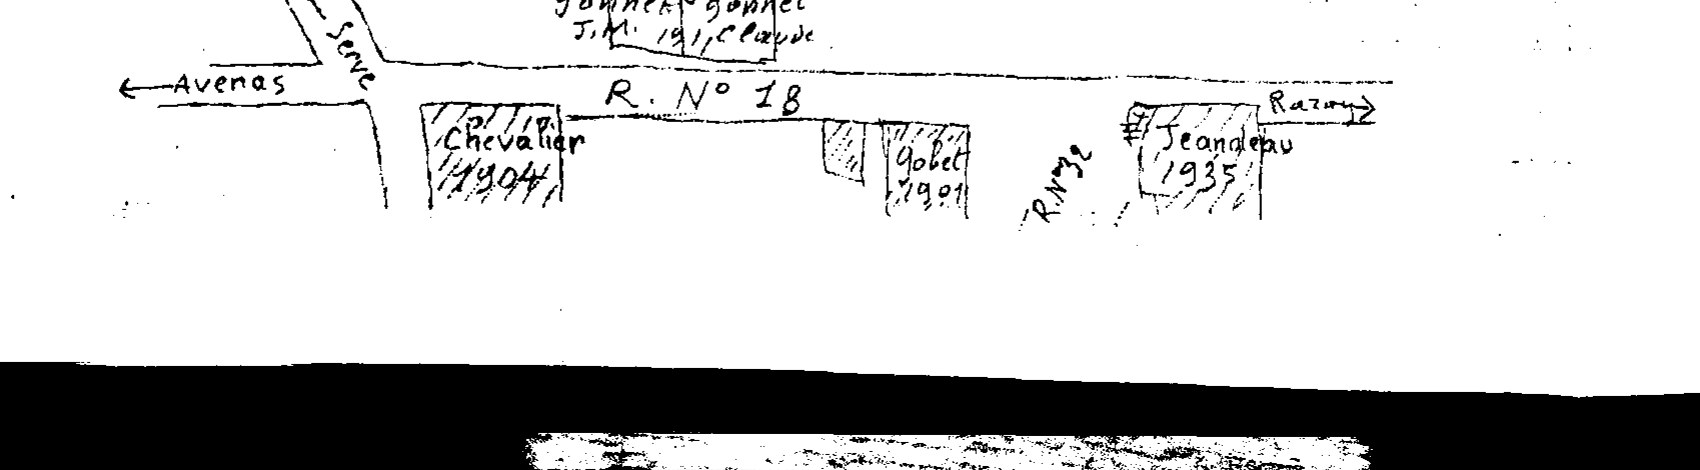
\includegraphics[width=0.62\textwidth]{Illustrations/illus-maisons-anciennes.jpg}\end{center}

% --- Page imprimée 271 — vue 274
\section*{Progrès social et matériel, par Jean BUFFIN de St-Mamert}
\addcontentsline{toc}{section}{Progrès social et matériel}

Si l'on compare ce qu'était la vie dans la commune d'Ouroux à la fin du siècle dernier avec la vie actuelle, on constate qu'un grand changement s'est produit tant au point de vue matériel qu'au point de vue social.

Les habitants d'Ouroux sont, comme tout bon Français qui se respecte, grognards et rouspéteurs, mais en réfléchissant ils doivent reconnaître que les changements qui se sont produits et auxquels ils ont largement contribué, sont nombreux.

Avant 1880, aucun moyen de communication n'existait. La gare la plus proche était Beaujeu. Si l'on voulait prendre le train, c'était à pied qu'il fallait franchir l'étape de 16 kilomètres. Le courrier était acheminé de Beaujeu par un service de voiture à cheval qui circulait de nuit et amenait ce dernier à Monsols où se faisait la répartition pour tout le canton.

Vers 1900, une ligne de chemin de fer départemental (surnommé le « tacot ») relia Villefranche à Monsols avec une station gare au col de Crie dont existent encore des vestiges (Voir note ci-dessous).

Dès lors, un service de voiture fut créé : Ouroux, Crie, Monsols qui faisait deux navettes par jour. Cette voiture amenait le courrier et transportait quelques voyageurs. C'était déjà une amélioration.

En 1909--1910 apparut la fée électricité et sa lumière jaillit dans le bourg. L'extension se fit petit à petit et à l'heure actuelle la commune entière est électrifiée.

Note. Il était aussi question de faire un embranchement de la ligne de chemin de fer du Col de Crie à Tramayes. Ce projet avait été adopté par le Conseil général du Rhône et celui de la Saône et Loire. Le conseil municipal d'Ouroux, sous la présidence de son maire, Mr Canard a tout fait, sans pouvoir aboutir, pour faire passer cette ligne de chemin de fer par Ouroux, St-Mamert, St-Jacques et Germolles. Dans le procès-verbal de la réunion du 24 novembre 1901 nous lisons :

« Le conseil proteste énergiquement contre le projet de la commission départementale indiquant la vallée de St-Christophe, pour le raccordement de Monsols à Tramayes. La vallée d'Ouroux compte 5 moulins, 2 scieries, 2 huileries, 2 fours à chaux et 3 tuileries. Ouroux a un bureau de poste et possède une étude de notaire. Autant de raisons qui militent en faveur d'une ligne de chemin de fer, même dans l'intérêt de cette ligne ». Ouroux n'obtint pas la ligne demandée.

% --- Page imprimée 272 — vue 275
La guerre de 1914--1918 marqua non seulement un temps d'arrêt dans la modernisation, mais elle lui enleva une grande partie de sa jeunesse. Il suffit de jeter un coup d'œil sur le monument aux morts !

En 1922, grâce au dévouement et à la perspicacité du maire, Mr Jean-Baptiste GONNET, un service journalier d'autobus fut créé, reliant Ouroux avec Belleville, ce qui transforma avantageusement la vie de la localité. (Qu'il nous soit permis d'apporter un hommage au maire de cette époque Mr Gonnet pour les améliorations faites dans la commune pendant l'exercice de ses mandats) (Voir note)

Point de vue social.

En 1886 un groupe d'habitants entreprit la création d'une société de secours mutuel. Elle fut fondée sous le titre de « L'UNION D'OUROUX » dont nous citerons simplement les noms des principaux animateurs formant le bureau : président : BENAIT Jean, forgeron ; vice-président : CANARD Alexandre, boulanger ; LAUJY Claude : trésorier ; GONNET J. B. secrétaire ; GOBET Jean : secrétaire adjoint. La tâche de ces mutualistes de la première heure fut laborieuse ; ils eurent beaucoup de mal à inspirer l'esprit mutualiste. Ceci fait, la Société alla toujours en progressant. En 1911 elle accepta dans son giron la petite commune de St-Mamert et prit le titre « L'UNION D'OUROUX et de SAINT MAMERT ». Au 1er Juillet 1930, en application de la loi sur les assurances sociales, elle créa dans son sein une section d'assurés sociaux agricoles. La gérance en fut confiée à un membre de son bureau : Mr Jean BUFFIN de St-Mamert.

----------------

Note. Avant de rappeler ce que la Commune doit à Mr « Gonnet J.B. » son ancien maire nommons ceux qui ont été placés à la tête de la commune : Mr LARGÉ ; Mr Adrien BERLOTY (de 1884 à 1897) ; Mr Alexandre CANARD (1897 à 1912) ; Mr VOLAND (1912--1917) ; Mr J.B. GONNET (1917 à 1934) ; Mr Félix BERLOTY (1935--1942) ; Mr J.B. GONNET fils (1942--1944) ; intérim assuré par Mr CL. MELINAND ; Mr J.M. BERTHET (1945--1952) ; intérim par Mr RAMPON qui a été élu maire.

Principaux travaux et améliorations faits sous le mandat de Mr J.B. GONNET : érection du monument sur la place et du caveau au cimetière, aux morts de la guerre ; érection de la salle des fêtes ; aménagement du cimetière ; création d'un service d'autobus ; élargissement du pont du fond du bourg ; installation d'un lavoir avec salle de bains-douches ; classement de la route de la Serve ; amélioration de la circulation dans le bourg ; électrification de la campagne ; etc. etc.

% --- Page imprimée 273 — vue 276
En 1903 fut créée une Mutuelle d'Assurance contre l'incendie, réassurée à la Caisse Régionale Incendie du Sud-Est, groupant les communes d'Ouroux, St-Mamert et St-Jacques-des-Arrêts, avec comme président : Mr Léon FIBOUL, propriétaire à la Carelle ; vice-président : Mr Alexandre CANARD ; secrétaire : Emile PRAT ; trésorier : MATRAY ; assesseurs : Jean-Baptiste GONNET, Jean Claude JOLY, Jean Louis JAMBON.

En 1925 fut créée une Coopérative de battage pour les communes d'Ouroux et St-Mamert avec comme président : Mr DUCARRÉ Claudius propriétaire à Ouroux ; vice-président : GONNET Jean-Baptiste ; secrétaire : BUFFIN Jean de St-Mamert ; trésorier : DESPERRIER Marius.

En 1932 fut créée une Mutuelle intercantonale contre la mortalité des chevaux, dont le siège est à Ouroux, avec comme président : Mr GOBET Claude, fermier à Ouroux ; vice-président : PASSOT Philibert, maire de St-Mamert ; BUFFIN Jean : secrétaire-trésorier ; GOBET Benoît : secrétaire-trésorier adjoint ; syndics : MM. PHILLET Marcel, GOBET J.M. GUIGNIER Louis ; ainsi que 2 assesseurs par commune ayant des membres à l'assurance.

En 1937 en exécution de la loi du 15-12-1922, rendant applicable à l'agriculture la loi de 1898 sur les accidents du travail, il fut créé une Caisse Mutuelle d'assurance contre les accidents, réassurée à la caisse régionale du Sud-Est avec Mr DUCARRÉ Claudius comme président ; Philibert PASSOT comme vice-président ; Marius JAMBON comme trésorier ; Jean BUFFIN comme secrétaire correspondant et Benoît GOBET, Claude LABRUYÈRE, Claudius THIBOULET, Aristide PASSOT comme administrateurs. Cette assurance groupe les communes d'Ouroux, St-Mamert et St-Jacques des Arrêts.

En 1941 les agriculteurs créèrent un syndicat agricole avec comme président Claude GOBET ; vice-président : Philibert AUFFRANC ; trésorier Marcel GAUTHIER ; secrétaire Maurice RICHONNIER. Cet organisme rend de grands services aux agriculteurs. Au point de vue moral, cela leur permet de se sentir les coudes des uns aux autres afin d'avoir plus de force pour défendre leurs intérêts. Au point de vue matériel, d'avoir des marchandises qui leur sont nécessaires à meilleur compte.

% --- Page imprimée 274 — vue 277
J'oubliais de signaler qu'en 1929 la « Caisse d'Epargne de Villefranche » installa à Ouroux une succursale de ses services qui sont très appréciés des économistes, sous la présidence de Mr le maire d'Ouroux, avec Melle MOULIN comme sous-caissière, et 24 administrateurs choisis dans les communes d'Ouroux, St-Mamert et St-Jacques.

En 1944 une Section intercommunale de l'Association des familles vit le jour, sous la responsabilité de Mr Claudius AUFFRANC, menuisier.

Si pendant une assez longue période, quoique bien troublée du fait de deux guerres en l'espace de 20 ans et dont la dernière a frisé la destruction, le progrès a marqué des points, il apparaîtrait qu'à l'heure actuelle, on fasse marche arrière. Au lieu d'avoir un service d'autobus tous les jours reliant Ouroux à Belleville et Ouroux à Tramayes avec deux navettes, celui-ci est totalement supprimé le dimanche, le mercredi et le vendredi. D'autre part le mardi et le jeudi il n'y a qu'une navette. Ces restrictions portent préjudice à la localité surtout l'été, Ouroux étant un site réputé pour les estivants.

Il faudrait à Ouroux l'adduction d'eau (on en parle ! Espérons que cela se réalisera !), une pompe à incendie (on en parla il fut un temps), un médecin, une pharmacie, un vétérinaire et une horloge à son clocher » J.B.
